\documentclass[../main.tex]{subfiles}
\graphicspath{{\subfix{../figures/}}}

\begin{document}
\section{迪米特法则(LoD)}
迪米特法则(Law of Demeter)又称为最少知识原则(一个对象应当对其他对象尽可能少的了解).

\textbf{迪米特法则的各种表述}:没有任何一个其他的OO设计法则有如此之多的表述方式,下面给出的是众多的表述中较有代表性 的几种.
\begin{itemize}
  \item 只与你直接的朋友们通信;
  \item 不要跟陌生人说话;
  \item 每一个软件模块对其他的模块都只有最少的知识,而且局限于那些与本模块密切相关的软件模块.
\end{itemize}
在上面的表述里面,什么是``直接'',``陌生''和``密切''则被有意识的模糊化了,以便在不同的环境下可以有不同的解释.
\subsection{狭义的迪米特法则}
如果两个类不必彼此直接通信,那么这两个类就不应当发生直接的相互作用,如果其中一个类需要调用另一个类的某一个方法的话,可以通过第三者转发这个调用.

\textbf{以下条件是成为``朋友''条件}:
\begin{itemize}
  \item 当前对象本身(this)
  \item 以参数形式传入到当前对象方法中的对象
  \item 当前对象的属性直接引用的对象
  \item 当前对象的属性如果是一个聚集,那么聚集中的元素也都是朋友
  \item 当前对象所创建的对象
\end{itemize}
\textbf{狭义的迪米特法则的缺点}:
\begin{itemize}
  \item 会在系统内造出大量的小方法,散落在系统的各个角落.这些方法仅仅是传递间接的调用, 并且与系统中的业务逻辑无关.
  \item 为了克服狭义迪米特法则的缺点,可以使用依赖倒转原则,引入一个抽象的类型引用``抽象陌生人''对象,使“A"依赖于``抽象陌生人C'',换言之,就是将``抽象陌生人C''变成朋友.
\end{itemize}
\textbf{不满足迪米特法则的设计}:
有三个类,分别是Someone,Friend和Stranger.其中Someone与Friend是朋友,而Friend与Stranger是朋友.相关类图如下所示:
\begin{figure}[H]
  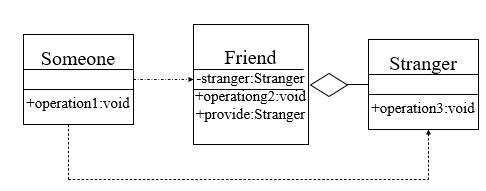
\includegraphics[width=0.55\textwidth]{14_1.jpg}
\end{figure}
\begin{lstlisting}[language=java]
// Someone
public class Someone {
  public void operation1(Friend friend) {
    Stranger stranger=friend.provide();
    stranger.operation3();
  }
}
\end{lstlisting}
\begin{lstlisting}[language=java]
// Friend
public class Friend {
  private Stranger stranger=new Stranger();
  public void operation2() {}
  public Stranger provide() {
    return stranger;
  }
}
\end{lstlisting}
显然,Someone的方法operation1()不满足迪米特法则.因为这个方法引用了Stranger对象,而Stranger对象不是Someone的朋友.

可以使用迪米特法则对上面的例子改造,改造的方法就是调用转发.改造后的情况如下图所示:
\begin{figure}[H]
  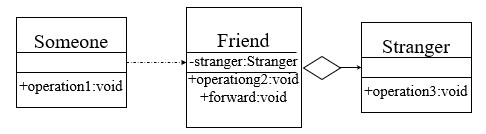
\includegraphics[width=0.55\textwidth]{14_2.jpg}
\end{figure}
\begin{lstlisting}[language=java]
// Someone
public class Someone {
  public void operation1(Friend friend) { friend.forward(); }
}
\end{lstlisting}
\begin{lstlisting}[language=java]
// Friend
public class Friend {
	private Stranger stranger=new Stranger();
	public void operation2() {
		System.out.println(“In Friend.operation2()”);
	}
	public void forward() {
		stranger.operation3();
	}
}
\end{lstlisting}
Friend类的forward()方法所做的就是以前Someone要做的事情,使用了Stranger的operation3()方法,而这种forward()方法叫做转发方法.
由于使用了调用转发,使得调用的具体细节被隐藏在Friend内部,从而使Someone与Stranger之间的直接联系被省略掉了.这样一来,使得系统内部的耦合度降低.在系统的某一个类需要修改时,仅仅会直接影响到这个类的朋友们,而不会直接影响到其余部分.
%
\subsection{广义的迪米特法则}
一个模块设计得好坏的一个重要的标志就是该模块在多大的程度上将自己的内部数据与实现有关的细节隐藏起来.
信息的隐藏非常重要的原因在于,它可以使各个子系统之间脱耦,从而允许它们独立地被开发,优化以及修改.
迪米特法则的主要用意是控制信息的过载.在运用迪米特法则到系统的设计中时,要注意以下几点:
\begin{itemize}
  \item 在类的划分上,应当创建弱耦合的类.类之间的耦合越弱,就越有利于复用.
  \item 在类的结构设计上,每一个类都应当尽量降低成员的访问权限.
  \item 在类的设计上,只要可能,一个类应当设计成不变类.
  \item 在对其他类的引用上,一个对象对其他对象的引用应降到最低.
  \item 尽量限制局部变量的有效范围.
\end{itemize}
\textbf{广义迪米特法则在类的设计上的体现}:
\begin{itemize}
  \item 优先考虑将一个类设置成不变类:
    Java语言的API中提供了很多的不变类,不变类易于设计,实现和使用.
    一个对象与外界的通信大体可以分为:改变这个对象的状态的和不改变这个对象的状态的.如果一个对象的内部状态根本就是不可能改变的,那么它与外界的通信自然也就大大减少了.
    当设计任何一个类的时候,都优先考虑这个类的状态是否需要改变.即便一个类必须是可变类,在给它的属性设置赋值方法的时候,也要保持谨慎的态度.除非真的需要,否则不要为一个属性设置赋值方法.
  \item 尽量降低一个类的访问权限:
    在满足一个系统对这个类的需求的同时,应当尽量降低这个类的访问权限.例如:
    \begin{enumerate}
      \item package-private:这是默认访问权限,如果一个类是package-private的,那么它就只能从当前库(包)访问.
      \item public:如果一个类是public的,那么这个类从当前库和其他库都可以访问.
    \end{enumerate}
\end{itemize}
\end{document}
